% Number 480
% UFPM Tension
% Accel. platform, 2 men hanging from it
% MIT

% Watermark
\AddToShipoutPicture*{\BackgroundPic}

\addtocounter {ProbNum} {1}

\begin{floatingfigure}[r]{.33\textwidth}
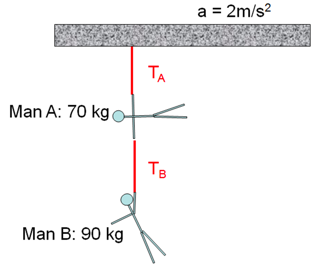
\includegraphics[scale=.6]{/Users/jgates/desktop/latex/pics/hangingmen}
\end{floatingfigure}
 
{\bf \Large{\arabic{ProbNum}}}Man A (70kg) and Man B (90kg) are hanging from a platform.  The platform accelerates upward at a constant rate of ${2~\tfrac{m}{s^2}}$. Assume that the ropes are massless. 

\bigskip
What is the tension in the top rope? Make a conceptual argument about why the size of this force makes sense.

%\begin{center}
%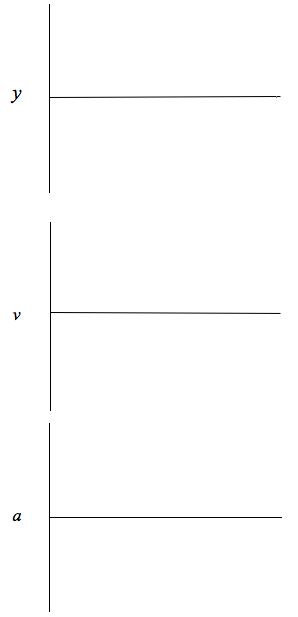
\includegraphics[scale=.85]{/Users/jgates/desktop/latex/pics/blankyvagraphstack.png}
%\end{center}


\vfill
\newpage
